

%*************************************************************************
% Chapter Quote
\begin{savequote}[50mm]
‘‘Equipado con sus cinco sentidos, el hombre explora el universo alrededor 
suyo y llama a esta aventura Ciencia’’
\qauthor{Edwin Hubble}
\end{savequote}
%*************************************************************************


\chapter{Introducción}
\label{cha:Introduction}

 
%*************************************************************************

‘‘¿Cuál es nuestro lugar en el cosmos?’’ Esta es una de las más simples
y trascendentales preguntas que siempre han acompañado a los seres humanos,
que además, potenciada por nuestra curiosidad innata nos ha conducido a
una imagen actual relativamente completa y entendible de nuestro universo.
De hecho, la astronomía solo puede ser considerada una disciplina científica
rigurosa después del siglo diecisiete.


%*************************************************************************





%*************************************************************************
%Prehistory
\section{Prehistoria}
\label{sec:Prehistory}


Casi en la mayoría de disciplinas científicas un avance teórico importante
viene acompañado de una mejora técnica de los instrumentos, es por esta 
razón que al comienzo del siglo diecisiete Johannes Kepler pudo establecer
sus tres bien conocidas leyes de movimiento planetario, basadas en los 
precisos datos de cuerpos astronómicos computados por Tycho Brahe. Este 
evento fue de gran importancia en la historia de la astronomía y la ciencia 
moderna debido a que fue el primero de muchos golpes contra la aceptada
noción antropocéntrica del cosmos. A pesar de estas leyes de Kepler 
constituían la prueba más crucial del modelo heliocéntrico de Nicolás 
Copérnico, fue solo hasta 1685 cuando Isaac Newton formulara su ley de 
gravitación universal (de las cuales pueden ser derivadas todas las leyes
de Kepler) cuando los astrónomos pudieron tener un conjunto de herramientas
teóricas suficientemente potentes para comenzar una discusión seria y 
profunda de la naturaleza real de nuestro universo a escalas mayores que el 
sistema solar, inaugurando así las \textit{ciencias de la gravedad} 
\cite{longair2008}.


Después de la formulación de la gravitación universal, el siguiente avance
teórico importante en esta área viene en los siglos dieciocho y diecinueve
con el desarrollo de la mecánica clásica, como el formalismo lagrangiano y
hamiltoniano, y de poderosas herramientas numéricas. Todos estos logros
impulsaron el estudio de temas claves como el problema de muchos cuerpos,
permitiendo un profundo entendimiento de la dinámica de sistemas 
gravitacionales complejos, tales como sistemas planetarios, cúmulos estelares,
etc.


Paralelo a lo anterior, en el lado observacional comenzaba a surgir la idea
de \textit{universo isla}, del cual evolucionaría el concepto de galaxia. 
Todo esto fue potenciado enormemente por el desarrollo del telescopio, 
permitiendo además entender que la galaxia es tan solo una gran colección
de estrellas tal como nuestro sol. Fue muy notable el trabajo pionero de 
William Herschel, quien intentó realizar un mapa de nuestra galaxia 
determinando distancias a partir de la asunción de estrellas con la misma
luminosidad intrínseca y la ley de inverso cuadrado para el decaimiento de 
la intensidad (figura \ref{fig:HerschelModel}). Aunque sus resultados
fueron muy imprecisos debido a la asunción incorrecta en que se basaban, 
la importancia de este trabajo radica en el reconocimiento de una estructura
(discoidal) de nuestra galaxia.


%.........................................................................
%Herschel Model of Our Galaxy
\begin{figure}[htbp]
	\centering
	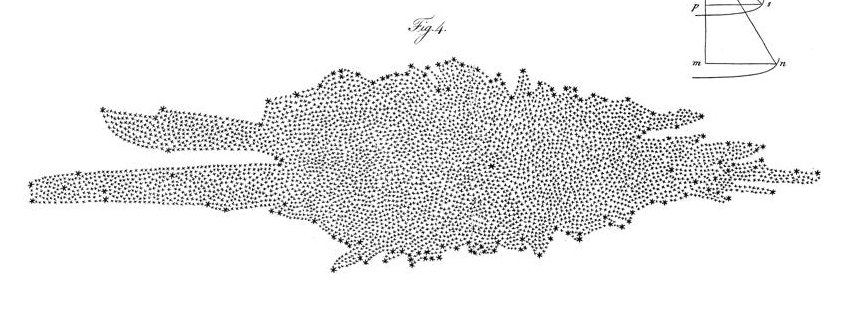
\includegraphics[width=1.0\textwidth]
	{./figures/1_introduction/Herschel_Model.png}
	
	\caption{\small{Modelo de William Herschel para nuestra galaxia, basado
	en un conteo de estrellas y la asunción de igual luminosidad \cite{Herschel1785}.}}
	
	\label{fig:HerschelModel}
\end{figure}
%.........................................................................


Otra importante cuestión observacional que estaba emergiendo en esa época
es sobre la existencia de otros \textit{universos islas} tal como el nuestro.
Era ya bien conocida la existencia de cuerpos extendidos en el cielo que no
se acomodaban satisfactoriamente a la definición de estrellas o planetas,
tales como nebulosas, discos planetarios y galaxias. Incluso William Herschel
y su hijo John Herschel contribuyeron con la realización de un gran catálogo
(para la época) de cuerpos extendidos conocido como \textit{Catálogo de 
Nebulosas y Cúmulos de Estrellas} y una versión expandida terminada por
John Dreyer en 1888, \textit{Nuevo Catálogo General de Nebulosas y Cúmulos
de Estrellas}, los cuales junto con el \textit{Índice de Catálogos} de 
1895 y 1908 constituyen una amplia colección de cuerpos ampliamente usados
en la astronomía actual, referidos con sus abreviaciones en inglés \textit{NGC}
y \textit{IC} respectivamente \cite{longair2008}. A pesar de todos estos
logros observacionales, la naturaleza real de estos objetos era un completo 
misterio, especialmente si ellos eran objetos dentro de nuestra propia 
galaxia o eran sistemas completamente independientes.


Esta última cuestión permaneció hasta el siglo veinte y junto con el tamaño
real del universo constituyeron los dos grandes temas tratados en el bien
conocido \textit{Gran Debate}, también denominado \textit{Debate de 
Shapley-Curtis}. Un importante evento en la historia de la astronomía donde
los astrónomos Harlow Shapley y Herber Curtis dieron respectivamente 
diferentes argumentos a favor y en contra de la pertenencia de esos objetos
a nuestra galaxia y si la Vía Láctea era todo nuestro universo. A pesar de 
todo, sus argumentos fueron poco concluyentes y la solución al estos 
problemas debió esperar hasta 1924 cuando Edwin Hubble midió la distancia
a la galaxia de Andrómeda (M31 o NGC 224) y demostró incuestionablemente 
la verdadera naturaleza extragaláctica de este objeto, y en años posteriores
para los demás. Este logro junto con la verificación observacional de la 
expansión del universo (también debida a Hubble) fueron el comienzo de la 
cosmología observacional moderna.


También sucedió en el siglo veinte un evento clave para las modernas 
\textit{ciencias de la gravedad}, Albert Einstein formuló su Teoría
General de la Relatividad, cambiando completamente la concepción previa
de espacio y tiempo, llegando así a nuestra compresión actual de la 
cosmología.


%*************************************************************************




%*************************************************************************
%The current cosmology picture
\section{La Cosmología Actualmente}
\label{sec:TheCurrentCosmologyPicture}


Las bases teóricas para la relatividad general comenzaron a surgir con el 
auge de las geometrías no Euclidianas en el siglo diecinueve y comienzos 
del veinte cuando fue demostrado que el quinto postulado de Euclides no 
era necesario para construir geometrías autoconsistentes, llegando así a las
geometrías no planas (ver figura \ref{fig:NonEuclidean}). En especial fueron 
destacables los trabajos de Nikolai Lobachevsky (padre de las geometrías 
no Euclideas) y Bernhard Riemman, fundador de la geometría Riemanniana.


%.........................................................................
%Herschel Model of Our Galaxy
\begin{figure}[htbp]
	\centering
	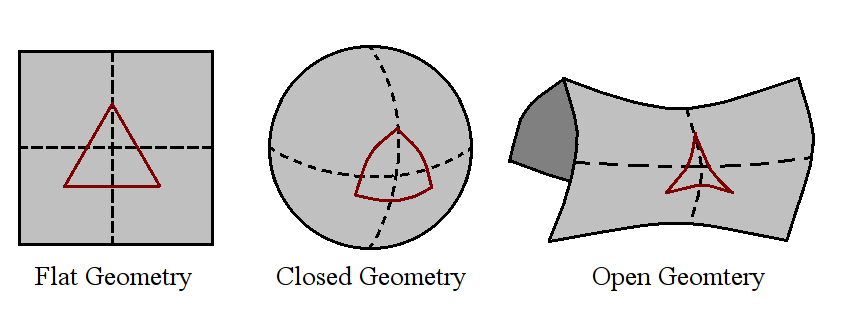
\includegraphics[width=0.9\textwidth]{./figures/1_introduction/Non_Euclidean.png}
	
	\caption{\small{Diferentes geometrías con variación del quinto postulado 
	de Euclides.}}
	
	\label{fig:NonEuclidean}
\end{figure}
%.........................................................................


A pesar de que estos primeros desarrollos en geometría había dado lugar a
fuertes discusiones sobre el tipo de geometría del universo, los conceptos de 
espacio y tiempo eran aún interpretados de forma absoluta y más aún, su 
conexión con la gravedad completamente ignorada. Es por esta razón que 
la formulación de la Relatividad General abrió la puerta a toda nuestra
comprensión moderna.


Una vez obtenidas las ecuaciones de campo métrico de la Relatividad General
fue posible construir modelos globales y autoconsistentes del universo. Un
primer intento se debe al propio Einstein, quién formuló con influencia 
de su propia creencia un modelo de universo estático y cerrado. Para lograr 
esto debió hacer uso de la bien conocida constante cosmológica para 
contrarrestar la expansión/contracción natural de las soluciones que dan 
la teoría.


Pocos años después	




%*************************************************************************

